% !TEX program = pdflatex
% ------------------------------------------------------------
% ITKA2004 Databases & Data Management
% Lecture: Schema Refinement and Normal Forms (90 min)
% Theme: metropolis (JYU-ish colors)
% Michael Emmerich, Professor of Intelligent Computing, PS Fellow
% Faculty of Information Technology, University of Jyväskylä
% ------------------------------------------------------------
\documentclass[10pt,aspectratio=169]{beamer}

\usetheme[
  progressbar=frametitle,
  numbering=fraction
]{metropolis}

% --- Packages
\usepackage[utf8]{inputenc}
\usepackage{etoolbox}
\usepackage{amsmath,amssymb}
\usepackage{booktabs}
\usepackage{xcolor}
\usepackage{tikz}
\usetikzlibrary{positioning,arrows.meta,shapes.geometric,calc,trees}
\usepackage{etoolbox}

% --- JYU-ish colors (adjust HEX if you have official codes)
\definecolor{JYUblue}{HTML}{003A70}    % dark blue
\definecolor{JYUorange}{HTML}{FF6A00}  % orange

% --- Metropolis palette / accents
\setbeamercolor{palette primary}{bg=JYUblue, fg=white}
\setbeamercolor{frametitle}{bg=JYUblue!6, fg=JYUblue}
\setbeamercolor{progress bar}{fg=JYUorange, bg=JYUblue!20}
\setbeamercolor{structure}{fg=JYUblue}
\setbeamercolor{alerted text}{fg=JYUorange}
\setbeamercolor{title}{fg=JYUblue}
\setbeamercolor{subtitle}{fg=JYUblue!85}

% --- Blocks: blue for theory, orange for examples
\setbeamercolor{block title}{bg=JYUblue, fg=white}
\setbeamercolor{block body}{bg=JYUblue!5, fg=black}
\setbeamercolor{block title example}{bg=JYUorange, fg=white}
\setbeamercolor{block body example}{bg=JYUorange!10, fg=black}
\setbeamercolor{block title alerted}{bg=black!75, fg=white}
\setbeamercolor{block body alerted}{bg=black!5, fg=black}

% --- Theorem/definition styling
\setbeamertemplate{theorems}[numbered]


\newtheorem{remark}{Remark}

% --- Example block convenience
\newenvironment{examplebox}[1][Example]{\begin{exampleblock}{#1}}{\end{exampleblock}}

% ------------------------------------------------------------
% Footer (Metropolis)
% ------------------------------------------------------------
\setbeamertemplate{frame footer}{%
  \tiny Michael Emmerich (Professor of Intelligent Computing, PS Fellow)\hfill Databases Spring 2026\hfill Faculty of Information Technology, University of Jyväskylä%
}

% --- Metadata
\title{Databases and Data Management}
\subtitle{Schema Refinement and Normal Forms}
\author{Michael Emmerich (Professor of Intelligent Computing, PS Fellow)}
\institute{Faculty of Information Technology\\University of Jyväskylä}
\date{Spring 2026}

\titlegraphic{%
  \begin{tikzpicture}[remember picture,overlay]
    \node[anchor=south east,opacity=0.10] at ([xshift=-2mm,yshift=2mm]current page.south east) {%
      \begin{tikzpicture}[scale=0.75]
        \draw[rounded corners=6pt,line width=2pt] (0,0) rectangle (5,3);
        \draw[line width=2pt] (0.6,2.4) -- (4.4,2.4);
        \node[text=JYUblue] at (2.5,1.6) {\Large NF};
      \end{tikzpicture}
    };
  \end{tikzpicture}%
}

% --- Convenience macros
\newcommand{\proj}{\pi}
\newcommand{\select}{\sigma}
\newcommand{\join}{\Join}
\newcommand{\closure}[1]{#1^{+}}
\newcommand{\fd}{\rightarrow}
\newcommand{\mvd}{\twoheadrightarrow}

% --- Tiny table helper
\newcommand{\tinytable}[1]{\scriptsize #1 \normalsize}

% --- Stickman macro (must be in preamble; not inside a frame)
\newcommand{\stickman}[4]{% x,y,scale,headsymbol
  \begin{scope}[shift={(#1,#2)}, scale=#3]
    \draw[line width=0.9pt] (0,0.25) circle (0.18);
    \node[font=\scriptsize] at (0,0.25) {#4};
    \draw[line width=0.9pt] (0,0.07) -- (0,-0.55);
    \draw[line width=0.9pt] (-0.32,-0.15) -- (0.32,-0.15);
    \draw[line width=0.9pt] (0,-0.55) -- (-0.28,-0.95);
    \draw[line width=0.9pt] (0,-0.55) -- (0.28,-0.95);
  \end{scope}
}

\begin{document}

\maketitle

% ------------------------------------------------------------
\begin{frame}{Today (90 minutes)}
\begin{itemize}
  \item The evils of redundancy; decomposition as remedy
  \item Functional dependencies (FDs) and reasoning (Armstrong)
  \item Keys and superkeys
  \item Normal forms: \textbf{BCNF} and \textbf{3NF} (and why we need them)
  \item Decomposition properties: lossless join and dependency preservation
  \item BCNF decomposition (algorithm + examples)
  \item 3NF: minimal cover and dependency-preserving refinement
  \item Multivalued dependencies and 4NF (brief)
\end{itemize}
\end{frame}

\begin{frame}{What we focus on (and what we skip)}
\begin{itemize}
  \item \textbf{1NF is trivial here}: we assume atomic attributes (no repeating groups / nested lists).
  \item \textbf{2NF is not needed for this course}: mainly historical and weaker than 3NF.
  \item We focus on \textbf{BCNF and 3NF} and why they are needed:
  \begin{itemize}
    \item diagnose redundancy using FDs and keys,
    \item refine safely via lossless join decomposition,
    \item understand the tradeoff between BCNF and dependency preservation.
  \end{itemize}
\end{itemize}
\end{frame}

\begin{frame}{Learning goals}
\begin{enumerate}
  \item Identify redundancy and anomalies; explain why decomposition can help
  \item Define FDs and reason with them (Armstrong + derived rules)
  \item Determine keys/superkeys; apply them to normal forms
  \item Check lossless join and dependency preservation
  \item Apply BCNF decomposition and understand non-uniqueness
  \item Explain why 3NF is sometimes preferred (dependency preservation)
  \item Recognize MVDs and the idea of 4NF
\end{enumerate}
\end{frame}

\begin{frame}{Outline}
\tableofcontents
\end{frame}

% ============================================================
\section{Redundancy and anomalies}

\begin{frame}{The evils of redundancy; decomposition as a remedy}
\begin{examplebox}[Example: schema with redundancy; decomposition]
The single-table schema \texttt{Client(cid, name, postcode, city, province)} has redundancy; dependences\\
\texttt{postcode}$\rightarrow$\texttt{city}, \ \texttt{city}$\rightarrow$\texttt{province}.\\[0.2em]
\(\Rightarrow\) Decompose into \texttt{Client(cid, name, postcode)}, \texttt{Place(postcode, city)}, \texttt{Cities(city, province)}.
\end{examplebox}

\begin{itemize}
  \item Redundancy causes: redundant storage, insert/delete/update anomalies.
  \item FDs can identify problematic schemas and suggest refinements.
  \item Main refinement technique: \textbf{decomposition}.
  \item Decomposition should be used judiciously: remove redundancy, avoid new problems.
\end{itemize}
\end{frame}

% --- Insert this slide right after the Outline (or right before the first redundancy slide)

\begin{frame}{Redundancy at a glance (why we care)}
\small
\begin{columns}[T,onlytextwidth]
\column{0.48\textwidth}
\begin{block}{What is redundancy?}
Storing the \emph{same fact} multiple times (explicitly or implicitly).\\
Often happens when a table mixes \emph{different kinds of facts}.
\end{block}

\begin{examplebox}[Toy example: repeated place facts]
\[
Client(cid,name,postcode,city,province)
\]
FDs (semantics):
\[
postcode \rightarrow city,\qquad city \rightarrow province
\]
So \((postcode,city)\) and \((city,province)\) repeat for many clients.
\end{examplebox}

\column{0.52\textwidth}
\begin{examplebox}[A tiny instance]
\scriptsize
\[
\begin{array}{|c|c|c|c|c|}\hline
cid&name&postcode&city&province\\\hline
1&anna&40100&jyvaskyla&central\_finland\\
2&ben&40100&jyvaskyla&central\_finland\\
3&cara&33100&tampere&pirkanmaa\\\hline
\end{array}
\]
\end{examplebox}

\begin{block}{What can go wrong?}
\begin{itemize}
  \item \textbf{Update Anomaly:} city/province rename must be changed in many rows
  \item \textbf{Insert Anomaly:} cannot store a new postcode without a client
  \item \textbf{Delete Anomaly:} deleting last client of a postcode loses the mapping
\end{itemize}
\end{block}
\end{columns}
\end{frame}

% ============================================================
\section{Functional dependencies}

\begin{frame}{Functional Dependences (FDs)}
\begin{definition}[Functional dependence]
A functional dependence \(X \rightarrow Y\) holds over relation \(R\) if, for every allowable instance \(r\) of \(R\),
for all tuples \(t_1,t_2\in r\):
\[
\proj_X(t_1)=\proj_X(t_2)\ \Rightarrow\ \proj_Y(t_1)=\proj_Y(t_2).
\]
\end{definition}

\begin{itemize}
  \item An FD is a statement about \emph{all allowable} relation instances.
  \item Must be identified from application semantics.
  \item From one instance you can detect violations, but not prove an FD holds.
  \item \(K\) is a candidate key means \(K \rightarrow R\); minimality is separate.
\end{itemize}
\end{frame}

\begin{frame}{Example: Hourly Employees}
\begin{examplebox}[An example relation]
\texttt{HourlyEmps(ssn, name, lot, rating, hourly\_wages, hours\_worked)}
\end{examplebox}

\begin{block}{Notation}
We abbreviate attributes as \(\textit{SNLRWH}\).
\end{block}

\texttt{Some FDs on Hourly\_Emps:}
\begin{itemize}
  \item ssn is the key: \(S \rightarrow \textit{SNLRWH}\)
  \item rating determines hourly wages: \(R \rightarrow W\)
\end{itemize}
\end{frame}

\begin{frame}{Redundancy caused by FDs and decomposition as a remedy}
\begin{columns}[T,onlytextwidth]
\column{0.48\textwidth}
\textbf{Redundancy problems (due to \(R \rightarrow W\))}
\begin{itemize}
  \item Update anomaly: can we change \(W\) in just the 1st tuple?
  \item Insertion anomaly: insert employee without wage for rating?
  \item Deletion anomaly: delete all rating-5 employees \(\Rightarrow\) lose wage for rating 5
\end{itemize}
\textbf{Remedy:} decompose into two tables: \texttt{Hourly\_Emps2} and \texttt{Wages}.

\column{0.52\textwidth}
\textbf{Relation instances (as tables)}\\[-0.2em]
\tinytable{
\[
\begin{array}{|c|c|c|c|c|c|}\hline
S & N & L & R & W & H\\\hline
123\!-\!22\!-\!3666 & attishoo & 48 & 8 & 10 & 40\\
231\!-\!31\!-\!5368 & smiley  & 22 & 8 & 10 & 30\\
131\!-\!24\!-\!3650 & smethurst & 35 & 5 & 7 & 30\\
434\!-\!26\!-\!3751 & guldu   & 35 & 5 & 7 & 32\\
612\!-\!67\!-\!4134 & madayan & 35 & 8 & 10 & 40\\\hline
\end{array}
\]
decomposes to:\\ 
\vspace{-0.4em}
\[
\mbox{Hourly\_Emps2} =
\begin{array}{|c|c|c|c|c|}\hline
S & N & L & R & H\\\hline
123\!-\!22\!-\!3666 & attishoo & 48 & 8 & 40\\
231\!-\!31\!-\!5368 & smiley  & 22 & 8 & 30\\
131\!-\!24\!-\!3650 & smethurst & 35 & 5 & 30\\
434\!-\!26\!-\!3751 & guldu   & 35 & 5 & 32\\
612\!-\!67\!-\!4134 & madayan & 35 & 8 & 40\\\hline
\end{array}
\]
\[
\mbox{Wages} =
\begin{array}{|c|c|}\hline
R & W\\\hline
8 & 10\\
5 & 7\\\hline
\end{array}
\]
}
\end{columns}
\end{frame}

% \begin{frame}{Refining an ER diagram to remove FD-caused redundancy (TikZ)}
% \begin{columns}[T,onlytextwidth]
% \column{0.35\textwidth}
% \begin{itemize}
%   \item If all employees in a department share the same parking lot, then:
%   \item remove attribute \texttt{lot} from \texttt{Employees}
%   \item add attribute \texttt{lot} to \texttt{Departments}
%   \item key constraint on \texttt{Works\_in} matters (each employee works in one dept).
% \end{itemize}

% \column{0.65\textwidth}
% \centering
% \begin{tikzpicture}[font=\scriptsize,
%   entity/.style={draw,rounded corners,minimum width=2.2cm,minimum height=0.8cm,align=center},
%   rel/.style={draw,diamond,aspect=2,inner sep=1.5pt,align=center},
%   attr/.style={draw,ellipse,inner sep=2.2pt},
%   edge/.style={-Latex,thick}
% ]
% % BEFORE
% \node[entity] (e1) at (0,1.9) {Employees};
% \node[entity] (d1) at (4.2,1.9) {Departments};
% \node[rel] (w1) at (2.1,1.9) {Works\_in};
% \draw[edge] (e1) -- (w1);
% \draw[edge] (w1) -- (d1);

% \node[attr] (ssn1) at (-1.6,2.6) {ssn};
% \node[attr] (name1) at (-1.6,1.9) {name};
% \node[attr] (lot1) at (-1.6,1.2) {lot};
% \draw (ssn1) -- (e1);
% \draw (name1) -- (e1);
% \draw (lot1) -- (e1);

% \node[attr] (did1) at (5.4,2.6) {did};
% \node[attr] (dname1) at (5.4,1.9) {dname};
% \node[attr] (bud1) at (5.4,1.2) {budget};
% \draw (did1) -- (d1);
% \draw (dname1) -- (d1);
% \draw (bud1) -- (d1);

% \node[font=\scriptsize, text=black!60] at (2.1,2.75) {before};

% % AFTER
% \node[entity] (e2) at (0,0.2) {Employees};
% \node[entity] (d2) at (4.2,0.2) {Departments};
% \node[rel] (w2) at (2.1,0.2) {Works\_in};
% \draw[edge] (e2) -- (w2);
% \draw[edge] (w2) -- (d2);

% \node[attr] (ssn2) at (-1.6,0.2) {ssn};
% \node[attr] (name2) at (-1.6,-0.6) {name};
% \draw (ssn2) -- (e2);
% \draw (name2) -- (e2);

% \node[attr] (did2) at (5.4,0.9) {did};
% \node[attr] (dname2) at (5.4,0.2) {dname};
% \node[attr] (bud2) at (5.4,-0.5) {budget};
% \node[attr] (lot2) at (5.4,-1.2) {lot};
% \draw (did2) -- (d2);
% \draw (dname2) -- (d2);
% \draw (bud2) -- (d2);
% \draw (lot2) -- (d2);

% \node[font=\scriptsize, text=black!60] at (2.1,1.05) {after};
% % key constraint hint
% \node[font=\scriptsize, text=black!65] at (2.1,-0.65) {key constraint on Works\_in};
% \end{tikzpicture}
% \end{columns}
% \end{frame}

% ============================================================
\section{Reasoning with FDs}

\begin{frame}{Closure of a set of FDs}
\begin{examplebox}[Example of implied FD]
Let \(R(\texttt{ssn},\texttt{did},\texttt{lot})\) with FDs
\(\texttt{ssn}\rightarrow\texttt{did}\) and \(\texttt{did}\rightarrow\texttt{lot}\).
Then also \(\texttt{ssn}\rightarrow\texttt{lot}\).
\end{examplebox}

\begin{definition}[Closure \(F^+\)]
Given a set \(F\) of FDs, its closure \(F^+\) is the set of all FDs implied by \(F\) (including those in \(F\)).
\end{definition}

\begin{remark}
To find implied FDs, we apply Armstrong's axioms.
\end{remark}
\end{frame}

\begin{frame}{Armstrong's axioms}
\begin{block}{Armstrong’s Axioms}
Let \(X,Y,Z\) denote sets of attributes:
\begin{itemize}
  \item Reflexivity: if \(Y \subseteq X\), then \(X \rightarrow Y\)
  \item Augmentation: if \(X \rightarrow Y\), then \(XZ \rightarrow YZ\) for any \(Z\)
  \item Transitivity: if \(X \rightarrow Y\) and \(Y \rightarrow Z\), then \(X \rightarrow Z\)
\end{itemize}
\end{block}

\begin{theorem}[Soundness and completeness]
Armstrong's axioms are sound and complete inference rules for FDs:
\begin{itemize}
  \item Sound: they generate only FDs in \(F^+\).
  \item Complete: repeated application generates all FDs in \(F^+\).
\end{itemize}
\end{theorem}
\end{frame}

\begin{frame}{Derived inference rules: union and decomposition}
\begin{theorem}[Additional rules (from Armstrong)]
\begin{itemize}
  \item Union: if \(X \rightarrow Y\) and \(X \rightarrow Z\), then \(X \rightarrow YZ\)
  \item Decomposition: if \(X \rightarrow YZ\), then \(X \rightarrow Y\) and \(X \rightarrow Z\)
\end{itemize}
\end{theorem}

\begin{examplebox}[Proof (Using Armstrong's Axioms)]
\small
Union: \(X \rightarrow XY\) (augmentation), \(XY \rightarrow YZ\) (augmentation), \(X \rightarrow YZ\) (transitivity).\\
Decomposition: \(YZ \rightarrow Y\), \(YZ \rightarrow Z\) (reflexivity), then \(X \rightarrow Y\) and \(X \rightarrow Z\) (transitivity).
\end{examplebox}

\begin{remark}
Also useful: if \(X \rightarrow Y\) and \(XY \rightarrow Z\), then \(X \rightarrow Z\). (Prove! Exercise.)
\end{remark}
\end{frame}

% ============================================================
\section{Lossless join, normal forms, keys}

\begin{frame}{Lossless join decompositions, normal forms, keys}
\centering\textbf{How shall we decompose a relation in order to avoid redundancy?}
\vspace{0.5em}
\begin{itemize}
  \item Preserve information: \textbf{lossless join decomposition}.
  \item Normal forms (BCNF, 3NF) reduce redundancy caused by FDs.
  \item Central notions: \textbf{key} and \textbf{superkey}.
\end{itemize}
\end{frame}

\begin{frame}{Key, superkey}
Let \(R\) be a relation schema with attribute set \(X\) and \(F\) a set of FDs.
\begin{block}{Superkey}
A \textbf{superkey} for \(R\) is a subset \(K \subseteq X\) such that \(K \rightarrow X\).
\end{block}
\begin{block}{(Minimal) key}
A \textbf{(minimal) key} for \(R\) is a subset \(K \subseteq X\) such that:
\begin{enumerate}
  \item \(K \rightarrow X\)
  \item no proper subset of \(K\) determines \(X\)
\end{enumerate}
\end{block}
\begin{alertblock}{Remarks}
\begin{itemize}
  \item Supersets of keys are superkeys; they are not minimal keys.
  \item A relation can have multiple candidate keys.
\end{itemize}
\end{alertblock}
\end{frame}

\begin{frame}{Some tricks to find keys}
\begin{block}{Right-hand side rule}
If an attribute never occurs on the RHS of any FD, it must belong to every key.
\end{block}
\begin{block}{Left-hand side rule}
If an attribute never occurs on the LHS but occurs on at least one RHS, it must not belong to any key.
\end{block}
\begin{block}{Start from small sets}
Search keys from small attribute sets and prune supersets of found keys.
\end{block}
\end{frame}

\begin{frame}{Boyce-Codd normal form and 3NF: the definitions}
\begin{block}{BCNF}
A relation schema \(R\) is in BCNF if for every non-trivial FD \(X \rightarrow Y\) in \(R\), where \(Y \nsubseteq X\),
\(X\) is a superkey of \(R\).
\end{block}

\begin{block}{3NF}
A relation schema \(R\) is in 3NF if for every non-trivial FD \(X \rightarrow Y\) in \(R\), where \(Y \nsubseteq X\),
\(X\) is a superkey of \(R\), or \(Y\) is part of a key of \(R\).
\end{block}

\begin{alertblock}{Remarks about normal forms}
\begin{itemize}
  \item To check BCNF/3NF: test all non-trivial FDs against the definition.
  \item BCNF implies 3NF.
  \item 1NF is trivial here; 2NF is mainly historical and weaker than 3NF.
  \item BCNF and 3NF are needed; we will decompose into them systematically.
\end{itemize}
\end{alertblock}
\end{frame}

% ============================================================
\section{Decomposition properties}

\begin{frame}{Decomposition: definition}
\begin{definition}[Decomposition]
Suppose relation \(R\) contains attributes \(A_1,\dots,A_n\). A decomposition replaces \(R\) by two or more relations such that:
\begin{itemize}
  \item each new schema contains a subset of attributes of \(R\),
  \item together they include all attributes in \(R\).
\end{itemize}
\end{definition}

\begin{examplebox}[Example]
\(\{AB,BCD,CD\}\) is a decomposition of \(ABCD\), whereas \(\{AB,BC\}\) is not.
\end{examplebox}

\begin{alertblock}{Potential problems}
\begin{itemize}
  \item some queries become more expensive (joins)
  \item may not be reconstructable (if not lossless)
  \item constraints may require joins to check (if not dependency-preserving)
\end{itemize}
\end{alertblock}
\end{frame}

\begin{frame}{Lossless join property (table example)}
\begin{block}{Lossless join decomposition}
Decomposition of \(R\) into \(X\) and \(Y\) is lossless-join w.r.t.\ \(F\) if for every instance \(r\models F\):
\[
\proj_X(r)\ \bowtie\ \proj_Y(r)\ =\ r.
\]
\end{block}

\begin{columns}[T,onlytextwidth]
\column{0.32\textwidth}
\textbf{Instance \(r(A,B,C)\)}\\[-0.3em]
\tinytable{
\[
r=
\begin{array}{|c|c|c|}\hline
A&B&C\\\hline
1&2&3\\
4&5&6\\
7&2&8\\\hline
\end{array}
\]
}

\column{0.32\textwidth}
\textbf{\(\proj_{AB}(r)\) and \(\proj_{BC}(r)\)}\\[-0.3em]
\tinytable{
\[
\proj_{AB}(r)=
\begin{array}{|c|c|}\hline
A&B\\\hline
1&2\\
4&5\\
7&2\\\hline
\end{array}
\qquad
\proj_{BC}(r)=
\begin{array}{|c|c|}\hline
B&C\\\hline
2&3\\
5&6\\
2&8\\\hline
\end{array}
\]
}

\column{0.36\textwidth}
\textbf{Join can create spurious tuples}\\[-0.3em]
\tinytable{
\[
\proj_{AB}(r)\bowtie\proj_{BC}(r)=
\begin{array}{|c|c|c|}\hline
A&B&C\\\hline
1&2&3\\
1&2&8\\
4&5&6\\
7&2&3\\
7&2&8\\\hline
\end{array}
\]
}
\end{columns}

\small So \(\proj_{AB}(r)\bowtie\proj_{BC}(r)\neq r\): decomposition \(\{AB,BC\}\) is \textbf{not} lossless.
\end{frame}

\begin{frame}{Lossless join decomposition theorem}
\begin{theorem}[Lossless join based on FD closure]
The decomposition of \(R\) into \(X\) and \(Y\) is lossless-join w.r.t.\ \(F\) iff \(F^+\) contains:
\[
X\cap Y \rightarrow X \quad\text{or}\quad X\cap Y \rightarrow Y.
\]
\end{theorem}

\begin{examplebox}[Example lossless join check]
Let \(R(ABCE)\) and \(F=\{C\rightarrow E\}\). Decomposition \(ABC,\ BCE\) is lossless because \(ABC\cap BCE = BC\) and \((BC\rightarrow BCE)\in F^+\).
\end{examplebox}

\begin{alertblock}{Corollary (for BCNF decomposition)}
If \(U\rightarrow V\) holds (with \(V\notin U\)), then decomposing \(R\) into \(UV\) and \(R - V\) is lossless-join.
\end{alertblock}
\end{frame}

% ============================================================
\section{BCNF decomposition}

\begin{frame}{Lossless-join decomposition into BCNF relations (algorithm)}
\begin{theorem}[Lossless-join BCNF decomposition]
The following algorithm derives a lossless join decomposition of \(R(X)\) into relations that are all in BCNF:
\begin{enumerate}
  \item If \(U \rightarrow Y\) violates BCNF, with \(U \subset X\) and \(Y \notin U\) a single attribute, then decompose \(R\) into \(X - Y\) and \(UY\).
  \item Repeat step 1 on each resulting relation until every relation is in BCNF.
\end{enumerate}
\end{theorem}
\end{frame}

\begin{frame}{BCNF decomposition as a tree}
\small
\begin{columns}[T,onlytextwidth]
\column{0.4\textwidth}
\begin{examplebox}[Task]
Decompose \(CSJDPQV\) with FDs:
\[
SD \rightarrow P,\qquad J \rightarrow S.
\]
\end{examplebox}
\begin{block}{Idea}
\begin{itemize}
  \item First decompose using \(SD\rightarrow P\).
  \item Then decompose the remaining non-BCNF part using \(J\rightarrow S\).
\end{itemize}
\end{block}

\column{0.56\textwidth}
\centering
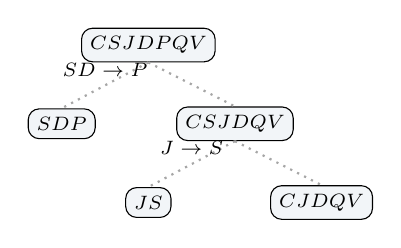
\begin{tikzpicture}[
  level distance=10mm,
  sibling distance=22mm,
  every node/.style={draw,rounded corners,align=center,inner sep=3pt,font=\scriptsize,fill=JYUblue!5},
  % disable the built-in tree edges (removes the strong black arcs)
  edge from parent/.style={draw=none}
]
% --- nodes (tree layout only) ---
\node (root) {\(CSJDPQV\)}
  child { node (sdp) {\(SDP\)} }
  child { node (csjdqv) {\(CSJDQV\)}
    child { node (js) {\(JS\)} }
    child { node (cjdqv) {\(CJDQV\)} }
  };

% --- custom connectors (drawn after layout; only these will appear) ---
\draw[dotted,gray!70,line width=0.8pt] (root.south) -- (sdp.north);
\draw[dotted,gray!70,line width=0.8pt] (root.south) -- (csjdqv.north);
\draw[dotted,gray!70,line width=0.8pt] (csjdqv.south) -- (js.north);
\draw[dotted,gray!70,line width=0.8pt] (csjdqv.south) -- (cjdqv.north);

% --- labels on top ---
\node[font=\scriptsize,fill=none,draw=none] at ($(root.south)!0.5!(sdp.north) + (0,2mm)$) {\(SD\rightarrow P\)};
\node[font=\scriptsize,fill=none,draw=none] at ($(csjdqv.south)!0.5!(js.north) + (0,2mm)$) {\(J\rightarrow S\)};
\end{tikzpicture}

\vspace{0.4em}
\scriptsize Resulting lossless decomposition: \(\{SDP,\ JS,\ CJDQV\}\) (all in BCNF).
\end{columns}
\end{frame}

\begin{frame}{Lossless join decomposition in BCNF (non-uniqueness example)}
\begin{alertblock}{Non-uniqueness of lossless join decomposition}
There can be different BCNF decompositions depending on which FD is used first.
\end{alertblock}

\begin{examplebox}[Example]
Decompose \(CSJDPQV\) with FDs \(\{SD \rightarrow P,\ J \rightarrow S\}\).
\end{examplebox}

\small
\begin{columns}[T,onlytextwidth]
\column{0.5\textwidth}
\centering
\textbf{Decompose first on \(SD\rightarrow P\)}
\medskip

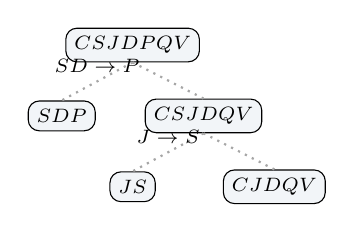
\begin{tikzpicture}[
  level distance=9mm,
  sibling distance=18mm,
  every node/.style={draw,rounded corners,align=center,inner sep=3pt,font=\scriptsize,fill=JYUblue!5},
  edge from parent/.style={draw=none} % suppress default black edges
]
\node (r1) {\(CSJDPQV\)}
  child { node (a1) {\(SDP\)} }
  child { node (b1) {\(CSJDQV\)}
    child { node (c1) {\(JS\)} }
    child { node (d1) {\(CJDQV\)} }
  };

% custom dotted connectors (no arrows)
\draw[dotted,gray!70,line width=0.8pt] (r1.south) -- (a1.north);
\draw[dotted,gray!70,line width=0.8pt] (r1.south) -- (b1.north);
\draw[dotted,gray!70,line width=0.8pt] (b1.south) -- (c1.north);
\draw[dotted,gray!70,line width=0.8pt] (b1.south) -- (d1.north);

% FD labels on top
\node[font=\scriptsize,fill=none,draw=none] at ($(r1.south)!0.5!(a1.north) + (0,2mm)$) {\(SD\rightarrow P\)};
\node[font=\scriptsize,fill=none,draw=none] at ($(b1.south)!0.5!(c1.north) + (0,2mm)$) {\(J\rightarrow S\)};
\end{tikzpicture}

\column{0.5\textwidth}
\centering
\textbf{Decompose first on \(J\rightarrow S\)}
\medskip

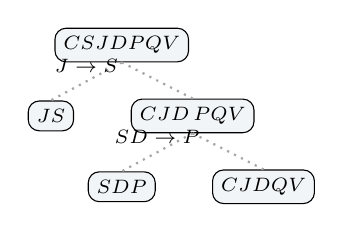
\begin{tikzpicture}[
  level distance=9mm,
  sibling distance=18mm,
  every node/.style={draw,rounded corners,align=center,inner sep=3pt,font=\scriptsize,fill=JYUblue!5},
  edge from parent/.style={draw=none} % suppress default black edges
]
\node (r2) {\(CSJDPQV\)}
  child { node (a2) {\(JS\)} }
  child { node (b2) {\(CJD\,PQV\)}
    child { node (c2) {\(SDP\)} }
    child { node (d2) {\(CJDQV\)} }
  };

% custom dotted connectors (no arrows)
\draw[dotted,gray!70,line width=0.8pt] (r2.south) -- (a2.north);
\draw[dotted,gray!70,line width=0.8pt] (r2.south) -- (b2.north);
\draw[dotted,gray!70,line width=0.8pt] (b2.south) -- (c2.north);
\draw[dotted,gray!70,line width=0.8pt] (b2.south) -- (d2.north);

% FD labels on top
\node[font=\scriptsize,fill=none,draw=none] at ($(r2.south)!0.5!(a2.north) + (0,2mm)$) {\(J\rightarrow S\)};
\node[font=\scriptsize,fill=none,draw=none] at ($(b2.south)!0.5!(c2.north) + (0,2mm)$) {\(SD\rightarrow P\)};
\end{tikzpicture}
\end{columns}

\vspace{0.2em}
\scriptsize Both are lossless; the intermediate relations differ.
\end{frame}

% ============================================================
\section{Dependency preservation and 3NF}

\begin{frame}{Dependence preserving property: theorems}
\begin{block}{Projection of a set of FDs}
If \(R\) is decomposed into \(X,\dots\), the projection of \(F\) onto \(X\) (denoted \(F_X\)) is the set of FDs \(U\rightarrow V\in F^+\) such that \(U,V\subseteq X\).
\end{block}

\begin{theorem}[Dependence preserving decomposition]
Decomposition of \(R\) into \(X\) and \(Y\) is dependence preserving iff
\[
(F_X \cup F_Y)^+ = F^+.
\]
\end{theorem}

\begin{examplebox}[Checking dependence preservation (as in the slides)]
Consider \(ABC\) with \(A\rightarrow B\), \(B\rightarrow C\), \(C\rightarrow A\), decomposed into \(AB\) and \(BC\).\\
\(C\rightarrow A\) is preserved: \(C\rightarrow B\) (from \(BC\)) and \(B\rightarrow A\) (from \(AB\)) \(\Rightarrow C\rightarrow A\).
\end{examplebox}
\end{frame}

\begin{frame}{Dependence preserving decomposition in 3NF: general procedure}
\begin{alertblock}{Existence}
It is not always possible to find a dependence-preserving decomposition in BCNF,
but it is always possible to find such a decomposition in 3NF.
\end{alertblock}

\begin{block}{Minimal cover \(F_0\) for a set of FDs \(F\)}
\begin{enumerate}
  \item \(F_0^+ = F^+\)
  \item RHS of each FD in \(F_0\) is a single attribute
  \item removing any FD (or LHS attribute) breaks property 1
\end{enumerate}
\end{block}

\begin{block}{General procedure (as in the slides)}
\begin{enumerate}
  \item Derive a minimal cover \(F_0\).
  \item Derive lossless join decomposition of \(R\) into BCNF relations.
  \item If some FD \(X\rightarrow Y \in F_0\) is not preserved, add relation \(XY\).
  \item Repeat step 3 until all FDs are preserved.
\end{enumerate}
\end{block}
\end{frame}

\begin{frame}{Algorithm to derive minimal cover}
\begin{block}{Procedure to derive minimal cover}
\begin{enumerate}
  \item Minimize RHS to single attributes (decomposition rule)
  \item Minimize LHS of FDs
  \item Remove redundant FDs (e.g., via transitivity)
\end{enumerate}
\end{block}

\begin{alertblock}{Remark on ordering}
The steps must be completed in the given ordering; different FD application orders can yield different minimal covers.
\end{alertblock}

\begin{examplebox}[Example (as in the slides)]
Example: \(AB \rightarrow CD,\ D\rightarrow E,\ A \rightarrow BE\).\\
Step 1: \(AB \rightarrow C,\ AB \rightarrow D,\ A \rightarrow B,\ A \rightarrow E\).\\
Step 2: \(AB \rightarrow C \Rightarrow A \rightarrow C,\ AB \rightarrow D \Rightarrow A \rightarrow D\).\\
Step 3: remove \(A \rightarrow E\) (since \(A \rightarrow D,\ D\rightarrow E\)).\\
Minimal cover: \(F_0=\{A \rightarrow C,\ A\rightarrow D,\ D\rightarrow E,\ A\rightarrow B\}\).
\end{examplebox}
\end{frame}

% ============================================================
\section{Multivalued dependencies and 4NF}

\begin{frame}{Multivalued dependences and higher order normal forms}
\begin{block}{Multivalued dependences}
An MVD exists when for each value of \(X\), the values of \(Y\) are independent of the values of \(R-X-Y\).
We write \(X \mvd Y\).
\end{block}

\begin{examplebox}[Delivery service]
Restaurant \(R\), Pizza Variety \(P\), Delivery Area \(D\).\\
\[
R \mvd P,\qquad R \mvd D.
\]
\end{examplebox}

\begin{block}{4NF (Fagin 1977)}
A table is in 4NF iff for every non-trivial MVD \(X \mvd Y\), \(X\) is a superkey.
\end{block}
\end{frame}

\begin{frame}{4NF example: redundancy from independent facts (table view)}
\scriptsize
\begin{columns}[T,onlytextwidth]
\column{0.54\textwidth}
\begin{examplebox}[Single table \((r,p,d)\)]
If varieties and areas are independent:
\[
r \mvd p,\qquad r \mvd d
\]
\end{examplebox}
\vspace{-0.2em}
\[
\begin{array}{|c|c|c|}\hline
r & p & d\\\hline
napoli & margherita & center\\
napoli & margherita & north\\
napoli & diavola    & center\\
napoli & diavola    & north\\\hline
\end{array}
\]

\column{0.46\textwidth}
\begin{examplebox}[4NF decomposition]
\[
rp(r,p)\quad\text{and}\quad rd(r,d)
\]
\end{examplebox}
\vspace{-0.2em}
\[
rp=\begin{array}{|c|c|}\hline
r & p\\\hline
napoli & margherita\\
napoli & diavola\\\hline
\end{array}
\qquad
rd=\begin{array}{|c|c|}\hline
r & d\\\hline
napoli & center\\
napoli & north\\\hline
\end{array}
\]
\end{columns}
\end{frame}

% ============================================================
\section{Wrap-up}

\begin{frame}{Take home messages}
\begin{itemize}
  \item Functional dependences and multivalued dependences are integrity constraints that can cause redundancy.
  \item Armstrong’s axioms and derived rules are key for reasoning with FDs (skill to practice).
  \item Decomposition into normal forms (3NF, BCNF, 4NF) can remove redundancy.
  \item Decompositions should ideally be lossless join (BCNF can always achieve this) and dependency preserving (3NF can always achieve this).
  \item Decomposition introduces joins; avoid unnecessary decomposition.
  \item Determination of keys is required to check normal forms; rules can guide.
  \item Two systematic procedures: BCNF decomposition (recursive tree) and 3NF via minimal cover.
\end{itemize}
\end{frame}

\begin{frame}{Quick self-check (exit ticket)}
\begin{enumerate}
  \item Why can BCNF fail to preserve dependencies, but 3NF can preserve them?
  \item State the binary lossless-join test in one line.
  \item Give one real-world example of redundancy causing an anomaly.
\end{enumerate}
\end{frame}

% ============================================================
\begin{frame}{Joke slide: Normalizing the relationship}
\small
\begin{columns}[T,onlytextwidth]
\column{0.56\textwidth}
A mess: the big kitchen table is gone. Now there are many small tables all over the kitchen.\\
The keys that were once neatly on the single kitchen table are distributed across them.\\[0.8em]
\textbf{Spouse:} ``Oh, darling, what did you do with the kitchen?!''\\[0.4em]
\textbf{Me:} ``No worries, Kulta, I just wanted to normalize our relationship.''\\[0.4em]
\textbf{Spouse:} ``...?''\\[0.8em]
\small (Moral: decomposition reduces redundancy, but too many relationships can make life complicated.)

\column{0.44\textwidth}
\centering
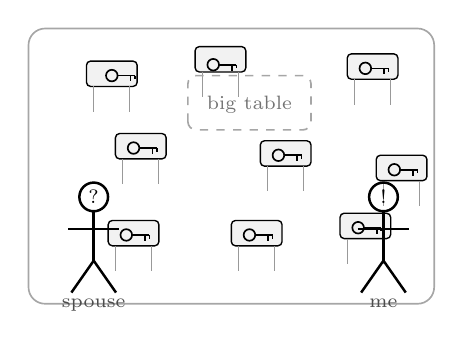
\begin{tikzpicture}[x=1cm,y=1cm,scale=0.92]

% kitchen boundary
\draw[rounded corners=6pt, line width=0.6pt, black!35] (-0.2,-0.2) rectangle (5.4,3.6);

% small tables scattered
\foreach \x/\y in {0.6/2.8, 2.1/3.0, 4.2/2.9, 1.0/1.8, 3.0/1.7, 4.6/1.5, 0.9/0.6, 2.6/0.6, 4.1/0.7} {
  \draw[fill=black!5, rounded corners=1.5pt, line width=0.5pt] (\x,\y) rectangle ++(0.7,0.35);
  \draw[line width=0.4pt, black!40] (\x+0.1,\y) -- (\x+0.1,\y-0.35);
  \draw[line width=0.4pt, black!40] (\x+0.6,\y) -- (\x+0.6,\y-0.35);
}

% keys scattered (simple key icon)
\foreach \x/\y in {0.95/2.95, 2.35/3.1, 4.45/3.05, 1.25/1.95, 3.25/1.85, 4.85/1.65, 1.15/0.75, 2.85/0.75, 4.35/0.85} {
  \draw[line width=0.6pt] (\x,\y) circle (0.08);
  \draw[line width=0.6pt] (\x+0.08,\y) -- (\x+0.32,\y);
  \draw[line width=0.6pt] (\x+0.26,\y) -- (\x+0.26,\y-0.08);
  \draw[line width=0.6pt] (\x+0.32,\y) -- (\x+0.32,\y-0.05);
}

% missing big table outline
\draw[dashed, line width=0.6pt, black!35, rounded corners=3pt] (2.0,2.2) rectangle (3.7,2.95);
\node[font=\scriptsize, text=black!55] at (2.85,2.55) {big table};

% spouse (?) and me (!)
\stickman{0.7}{1.0}{1.1}{?}
\stickman{4.7}{1.0}{1.1}{!}
\node[anchor=north, font=\scriptsize, text=black!70] at (0.7,0.0) {spouse};
\node[anchor=north, font=\scriptsize, text=black!70] at (4.7,0.0) {me};

\end{tikzpicture}
\end{columns}
\end{frame}

\end{document}